\cleardoublepage
\chapter{{Desarrollo Colaborativo de Productos CAD con Lean UX}}
\label{chap:cap3}

En este capítulo se explican los conceptos que involucran el desarrollo de los sistemas colaborativos y distribuidos para CAD y la metodología \textit{Lean UX} como una herramienta de soporte para desarrollar un software con tales características. Finalmente se describen algunos ejemplos de aplicaciones CAD colaborativas y distribuidas disponibles en la web.\vskip 0mm

\section{Introducción}
La complejidad creciente de los productos hace necesaria 
la colaboración entre diferentes personas, habitualmente se generalizan  en ``cliente'' y ``diseñador'' a las partes que interactúan, pero no necesariamente son una única persona por cada parte, 
sino equipos conformados por múltiples roles. Sus diferentes habilidades pueden abarcar el modelado 3D, la producción física con diferentes tecnologías (impresión 3D, corte a láser, control numérico, etc.), el marketing, etc. \vskip  

Tradicionalmente, la interacción se producía entregando los planos a  ``contratistas'' para que construyan las distintas partes que integran un proyecto, los contactos se producían de forma presencial y obligaban a frecuentes viajes para mantener el proyecto bajo control \citep{Ruiz}. Esta modalidad de trabajo se caracteriza por utilizar un \textbf{modelo en cascada}, que ordena rigurosamente las etapas del ciclo de vida de un proyecto, de tal forma que el inicio de cada etapa debe esperar a la finalización de la  anterior \citep{de2001metodologia}. Este modelo tiene la ventaja de ser sencillo de comprender e implementar, ya que se sabe de antemano que esperar del proyecto, con una estimación precisa del costo y  duración.
Sin embargo, una vez que un producto se encuentra en la etapa de prueba o revisión, es muy difícil realizar algún cambio por algo que no fue definido adecuadamente. De modo que el riesgo y la incertidumbre son elevados en los proyectos donde los requerimientos cambian constantemente. Por otro lado, no se distingue en involucrar al usuario final o cliente durante el proceso, si se solicita algún cambio no previsto, el proyecto se puede retrasar y salirse del presupuesto.\vskip
El avance de las tecnologías web ha democratizado la participación en los procesos de diseño en muchos niveles. Los teléfonos inteligentes son un ejemplo de la tecnología al servicio de las personas, porque ofrecen oportunidades para la co-creación mediante sus aplicaciones \citep{Huerta2013}. En consecuencia, el rol del contratista tradicional ha cambiado y esto implica que realice su trabajo en estrecha relación con otros actores, en colaboración y  sin necesidad del contacto presencial. En este nuevo escenario, la aparición de conceptos como \textbf{Desarrollo Colaborativo de Productos} en inglés \textit{Collaborative Product Development} (CPD) \citep{Elfving2007} impulsan la participación de ingenieros, diseñadores industriales, arquitectos, programadores, artistas e incluso personas sin formación específica en procesos conocidos como \textbf{co-diseño} o \textbf{diseño colaborativo}.

\section{Co-diseño}
 Se entiende como \textbf{co-diseño} al  proceso de colaboración creativa entre diseñadores y otras personas, las cuáles no poseen una formación previa en diseño, con el propósito de resolver problemas  \citep{PerezGarcia2014}.  
 En esta definición se plantean dos elementos fundamentales que dan soporte al paradigma colaborativo:
\begin{enumerate}
    \item \textbf{Nuevos perfiles}: Al grupo habitual de trabajo se suman la iniciativa y la creatividad de otros perfiles que antes aportaban ideas generalmente como agentes externos: el investigador y el usuario final. Estos perfiles tienden a mezclarse: El usuario pasa a jugar un rol de ``experto en su experiencia'' y puede aportar elementos de valor en la generación de conceptos e ideas en la etapa inicial del proyecto. El investigador, a partir de la experiencia del usuario, puede  recoger todos los datos y, a la vez, desempeñar un papel fundamental en formalizar las ideas. Lógicamente, una misma persona puede cumplir más de un rol y el diseñador debe cambiar al incluir nuevos ``socios creativos'' en un entorno que tradicionalmente le pertenecía.\vskip
\item \textbf{Objetivo en común}: La idea del \textbf{objetivo compartido} se plantea como una de las principales diferencias con respecto a los métodos tradicionales. Los métodos de diseño generalmente se planteaban para ser llevados a cabo solamente por expertos que realizaban tareas individuales y no era necesario compartir la visión del objetivo general del proceso. En cambio, en un proyecto colaborativo este punto es fundamental: Para que el equipo funcione correctamente necesita tener la visión del objetivo en común \citep{Huerta2013}.

\end{enumerate}


En la figura \ref{fig:codesign} se pueden apreciar las diferencias entre un esquema de \textbf{diseño tradicional vs co-diseño} \citep{Sanders2008}. En el esquema de la izquierda (tradicional) los roles trabajan por separado, el investigador aporta conocimientos para realizar la lista de requerimientos de diseño, la interacción del diseñador (contratista) con el usuario es a través de dicha lista. De esa manera el diseñador trabaja en base a los requerimientos y una vez finalizado todo el trabajo recién se efectúa la entrega. \vskip
Por otra parte, en el esquema de la derecha (co-diseño) el usuario participa durante todo el proceso de diseño a través de la  interacción directa con todo el equipo, en este ejemplo, el contratista cumple el rol de diseñador e investigador. La  interacción se realiza mediante las herramientas inherentes a cada proyecto, que pueden ser diagramas, referencias, artefactos, métodos y/o técnicas. En lugar de establecer los requerimientos, se plantean las necesidades de diseño y las entregas del trabajo se realizan progresivamente mediante la revisión continua del producto por parte de todos los participantes. 


\begin{figure}[h]
\centering
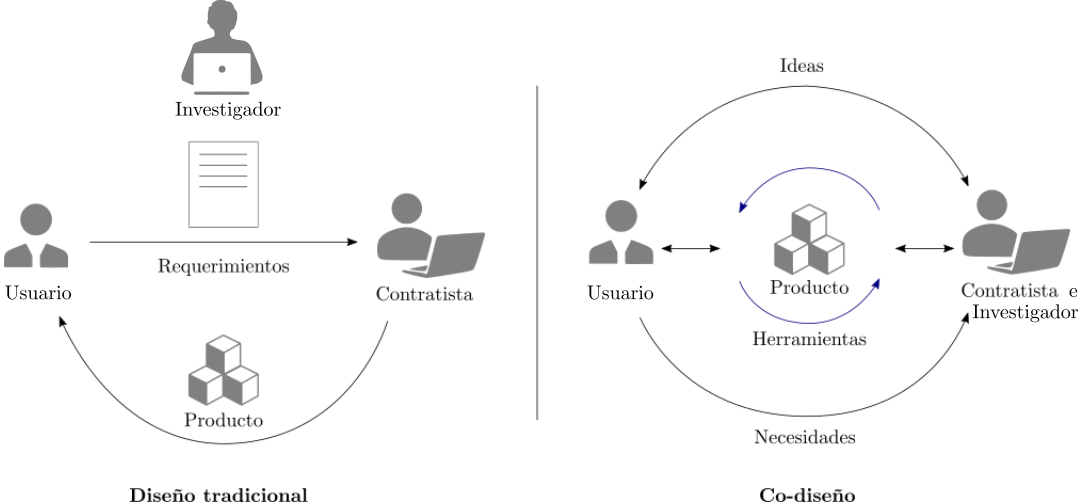
\includegraphics[width=16cm]{Img/INTRO/intro-codesign0.png}
\caption{\footnotesize{Diseño tradicional vs co-diseño.}}
\label{fig:codesign}
\end{figure}


La diversidad de profesiones en el co-diseño trae como consecuencia que los actores difieran tanto en la forma de interpretar el diseño como en la forma de comunicarlo. Generalmente la comunicación está cargada de jerga propia de cada especialidad y por lo tanto, es difícil de comprender para los demás participantes. Aun así, si se comprendieran las palabras, el significado de las mismas puede diferir según la disciplina. Un ejemplo de palabra con muchos significados es \textit{``concepto''}, la figura \ref{fig:concept} muestra cómo los actores de diferentes especialidades interpretan de diferente manera la misma palabra en el ambito de la industria automotriz: 
a) Para un diseñador son los dibujos rápidos, bosquejos o \textit{sketches}. b) Un fabricante de prototipos lo materializa en modelos de arcilla u otro material que permita visualizar rápidamente los detalles del producto, incluso en escala real. c) Para un publicista es la representación digital o render del producto final. d) Un ingeniero mecánico lo entiende en los documentos técnicos, planos y especificaciones. \citep{Kleinsmann2006} \\

En consecuencia, si no se crea un entendimiento compartido sobre el contenido del diseño, se dificulta la colaboración. 

\begin{figure}[ht]
\centering
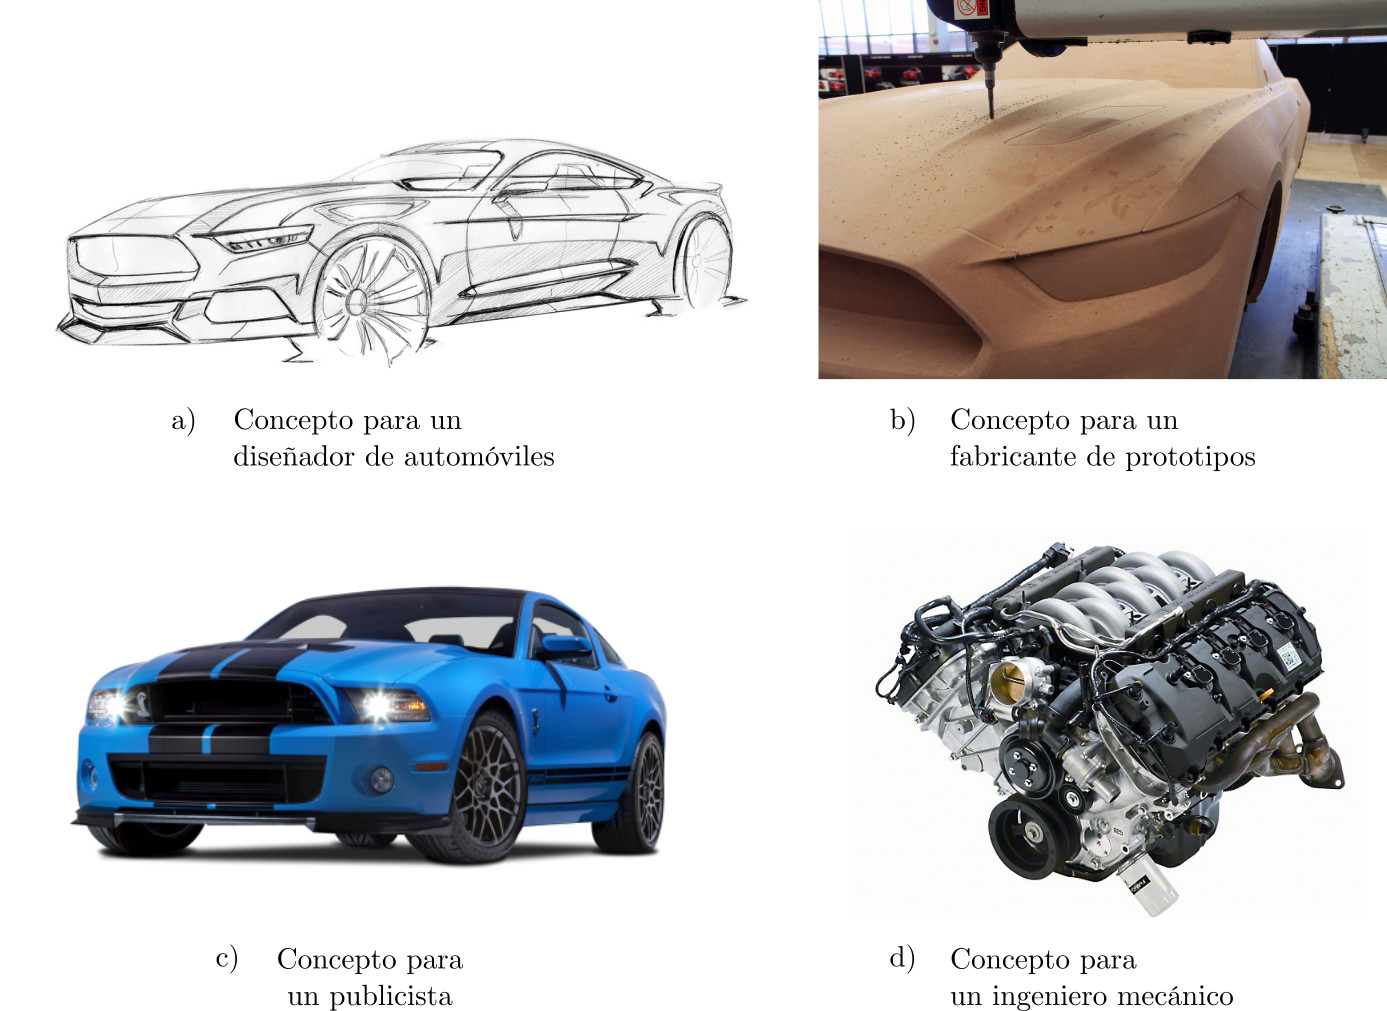
\includegraphics[width=14cm]{Img/INTRO/intro-codesign1.jpg}
\caption{\footnotesize{Interpretación de la palabra ``concepto" según especialistas de la industria automotriz.}}
\label{fig:concept}
\end{figure}

\subsubsection{Diseño Iterativo}
\label{iterativo}

La etapa de \textbf{revisión de los diseños} es fundamental porque permite evaluar la capacidad de los resultados para cumplir los requisitos del cliente, identificar cualquier problema y proponer soluciones \citep{Pereiro2005}. 

Lo más habitual es registrar los resultados de las revisiones en actas de reunión o bien en algún formato que se haya establecido  específicamente para el control. 
Estas tareas parecieran ser anticuadas en términos administrativos, si no se considera que diseñar un objeto tangible implica tener un entendimiento completo de todo lo que se debe hacer antes de iniciar la producción física, porque esta generalmente es compleja comparada con la producción de bienes intangibles. Por lo que la necesidad de la revisión constante y la tendencia creciente a requerimientos que pueden cambiar, ponen en evidencia las limitaciones del modelo en cascada. Como solución surgieron los \textbf{modelos iterativos} que promueven una iteración continua sobre el producto y pruebas a lo largo de todo el proyecto  \citep{laurel2003design}.

El \textbf{diseño iterativo} en inglés \textit{Iterative Design} es una metodología de diseño basada en un proceso cíclico de creación de prototipos\footnote{Un prototipo es un ejemplar o primer molde en que se fabrica una figura u otra cosa.} y pruebas, para analizar y refinar un trabajo que se encuentra en progreso. La interacción con el diseño se utiliza como una herramienta de investigación para recolectar información y desarrollar el proyecto, implementando iteraciones o versiones sucesivas. La prueba, el análisis, el refinamiento y la repetición son necesarios porque la experiencia del usuario no se puede predecir por completo. Las decisiones se basan en la experimentación  con el prototipo, de esta manera el proyecto se desarrolla a través de un continuo diálogo entre los diseñadores, el diseño y el usuario. 

\vskip
En un nivel superficial, el diseño iterativo  difiere del modelo de cascada de una sola manera: en lugar de especificar todo el sistema completo antes de desarrollarlo, se diseña y construye completamente una parte del mismo, y luego se utiliza esa parte y las unidades completadas previamente como base para más diseños y más producción futura. En otras palabras, \textbf{iterar es diseñar} y, específicamente, es comprender el diseño en el momento que se construye el diseño \citep{Chronicles2009}.\vskip




En este punto es necesario hacer una aclaración respecto a otro concepto con el que se suele confundir: \textbf{el diseño incremental} que tiene como objetivo un crecimiento progresivo de la funcionalidad. Es decir, el producto va evolucionando con cada una de las entregas hasta que se adapta a lo requerido por el cliente. Alistair Cockburn describe al enfoque iterativo como ``aprender al completar'' y lo distingue del diseño incremental en el sentido que éste consiste en agregar nuevos elementos, incluso de forma iterativa, mientras que iterar trata sobre volver a trabajar y refinar \citep{cockburn2002agile}. En ocasiones el concepto de iteración se puede perder al reemplazarlo por incrementos, lo que provoca que el proyecto tenga las mismas consecuencias que los en cascada. Jeff Patton, utilizando visualmente el cuadro de la Mona Lisa (ver figura \ref{fig: incremental}) para explicar la diferencia entre los dos métodos \citep{Patton2007}. En el incremental (arriba) se agregan nuevos elementos a partir de una idea completa preconcebida del producto. En el iterativo (abajo) se parte de una idea vaga, ejemplo: ``Una mujer en un ambiente campestre''. De forma iterativa se comienza a trabajar sobre una versión mínima del producto, refinando en cada ciclo hasta llegar a la solución.
Lo más destacado del método iterativo es el siguiente principio subyacente: Hasta que se no se haya construido realmente lo que se está diseñando, no se podrá comprender en su totalidad.

\begin{figure}[ht]
\centering
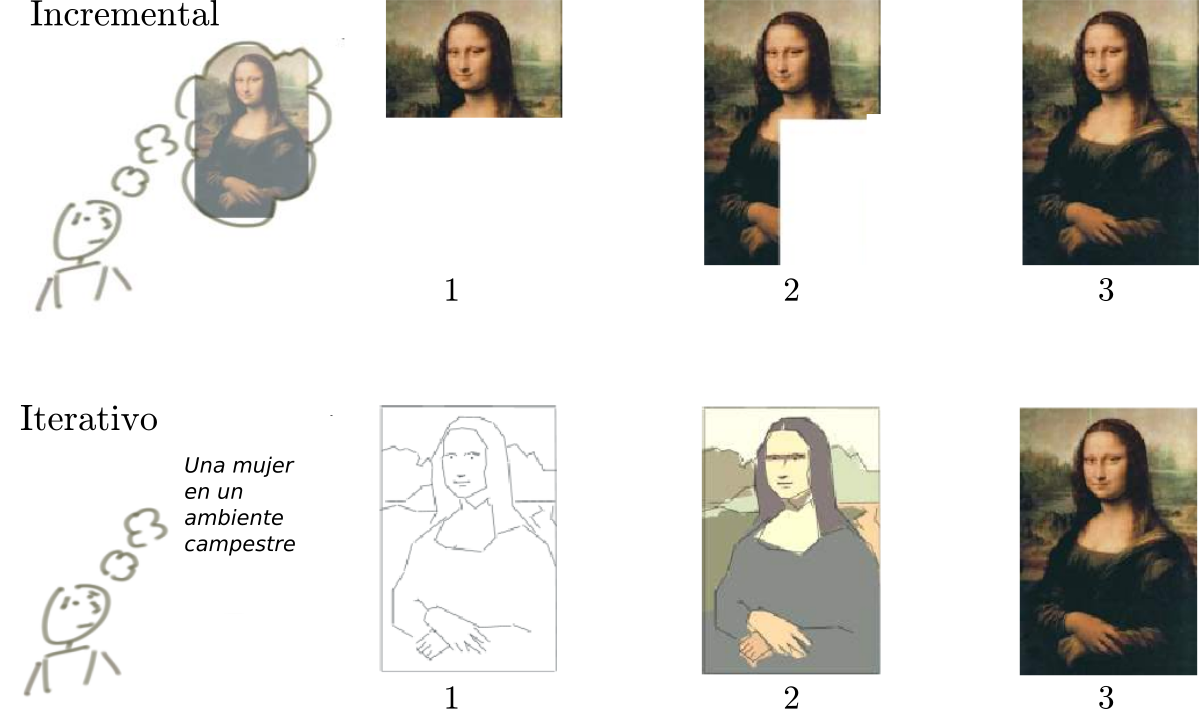
\includegraphics[width=12cm]{Img/CPD/mona.png}
\caption{\footnotesize{Diseño incremental vs iterativo.  }}
\label{fig: incremental}
\end{figure}


El concepto de iterativo se ha extendido con éxito a otras áreas como las metodologías \textit{\Gls{Agile}}  \citep{cockburn2002agile}.  
Por ejemplo, el marco de desarrollo \textit{\Gls{SCRUM}}\citep{Schwaber95scrumdevelopment} introduce el concepto de \textit{\Gls{sprint}}\footnote{Un Sprint, es un intervalo prefijado durante el cual se crea un incremento de producto ``Hecho o Terminado'' utilizable, potencialmente entregable} para referirse a la iteración.



\vskip


\subsubsection{Riesgo de la metodología en cascada frente a las iterativas}

{En este contexto, el riesgo se refiere a los factores que contribuyen al éxito o fracaso de un proyecto}. 
Todos los proyectos tienen algún riesgo, independientemente de su enfoque. En algunas situaciones, los factores inesperados que impactan positivamente el proyecto también son riesgos, pero se consideran  oportunidades.
Una regla que se aplica siempre es que \textbf{los riesgos negativos deben detectarse y mitigarse} \citep{layton2015scrum}. 

En la metodología en cascada existen una serie de factores negativos, propios de su estructura secuencial.
Un caso se puede analizar en la parte superior de la figura \ref{fig:water0} un modelo en cascada con las etapas \textit{definir, construir, testear y lanzar} para el desarrollo de un producto. Testear (probar) el producto justo antes del lanzamiento significa que si se presentan problemas en esa instancia se pone en riesgo todo el proyecto, la curva de riesgo incrementa notablemente justo al final de proyecto, en el lanzamiento. Por otro lado, en la parte inferior (ver figura \ref{fig:water0})  
se aprecia un modelo iterativo (Agile) con las mismas etapas definidas en todas las iteraciones. Si una decisión técnica, un requisito o incluso un producto completo no es factible, el equipo descubre esto en poco tiempo, por ende se cuenta con más tiempo para realizar correcciones. Si la corrección no es posible, de todas maneras el riesgo por el proyecto fallido es menor que con el enfoque en cascada \citep{Kukhnavets2016}.\vskip

\begin{figure}[ht]
\centering
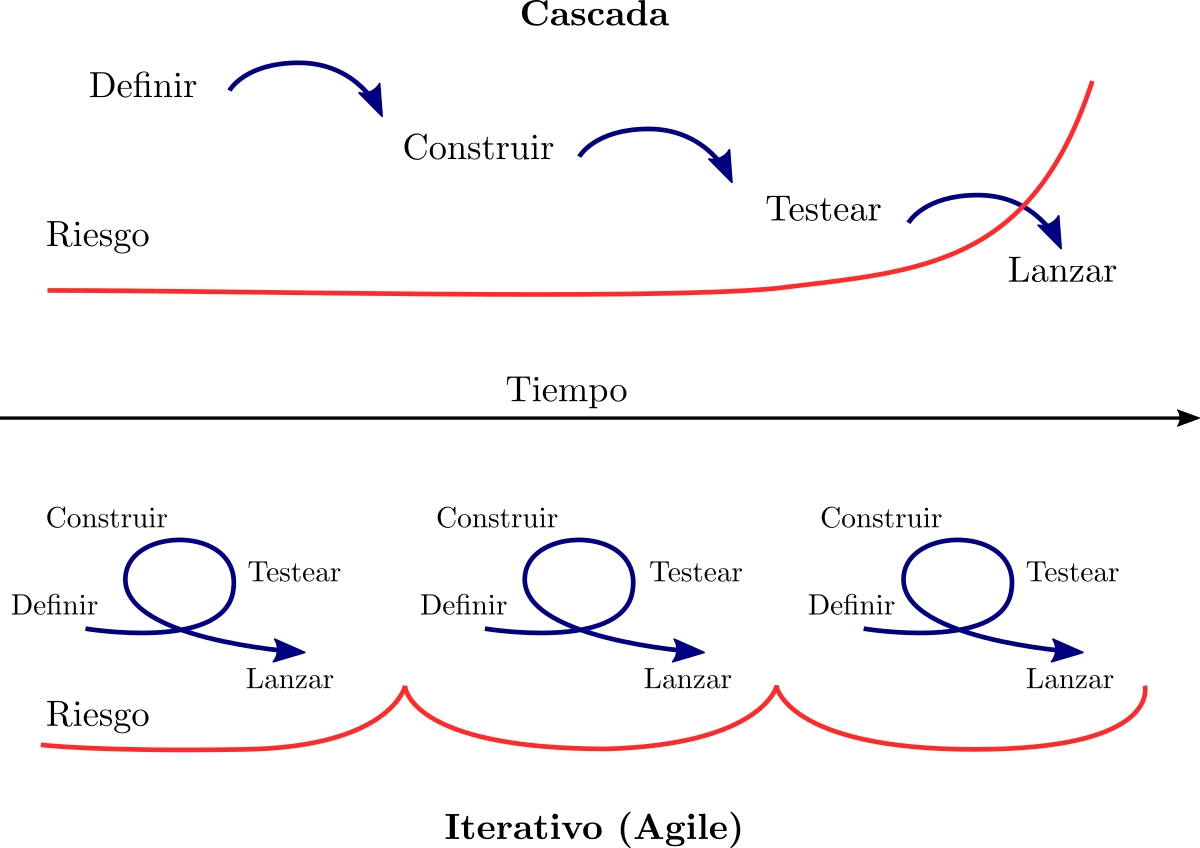
\includegraphics[width=13cm]{Img/CPD/cpd-water1.png}
\caption{\footnotesize{Riesgo de un proyecto en cascada vs iterativo (Agile).}}
\label{fig:water0}
\end{figure}
\vskip




Son evidentes las ventajas de la iteración y esto ha promovido que los nuevos productos se lancen a un ritmo creciente. Adicionalmente, tanto el hardware como el software evolucionaron para admitir la comunicación y el acceso multiusuario a los datos de diseño, la forma de acceso varía desde archivos compartidos hasta accesos compartidos mediante \textbf{Sistemas de Gestión de Bases de Datos} en inglés \textit{Data Base Management System} (\Gls{DBMS}) \citep{silberschatz2006fundamentos}. \vskip

Las aplicaciones CAD colaborativas se pueden identificar mediante una matriz (ver figura  \ref{fig:tablacad}) según su forma de uso en el tiempo y espacio \citep{Maher1997}. A continuación se analiza las diferentes configuraciones de la matriz.

\begin{enumerate}
    \item En el \textbf{mismo sitio y al mismo tiempo} es posible con una interfaz para un solo usuario, los diseñadores pueden compartir la misma computadora si necesitan colaborar.
    \item En el \textbf{mismo sitio pero en tiempos diferentes} es posible gracias a la gestión de datos técnicos, de manera que estén disponibles para la misma persona u otros miembros del equipo luego de que el diseño se completa.
    \item Al \textbf{mismo tiempo en sitios diferentes} se denomina 
    \textbf{CAD colaborativo} o bien \textbf{Co-Diseño}, diferentes diseñadores pueden ver y modificar el diseño en diferentes ubicaciones, viendo la misma imagen en la pantalla y comunicándose entre sí.
    \item En \textbf{sitios diferentes en tiempos diferentes} por consecuencia de la distribución de datos del diseño a través de una red (\textbf{CAD distribuido}), permitiendo a los actores acceder a los diseños independientemente de su ubicación y disponibilidad.
\end{enumerate}


La colaboración implica que el soporte informático (sistemas CAD) debe proporcionar flexibilidad en la comunicación de datos e ideas, considerando que el diseño colaborativo involucra muchos tipos de conocimiento de diferentes dominios. A continuación se analiza la forma en que los sistemas soportan estos paradigmas.


\vskip
\section{Sistemas CAD colaborativos}
\label{section:colabo}

\begin{figure}[ht]
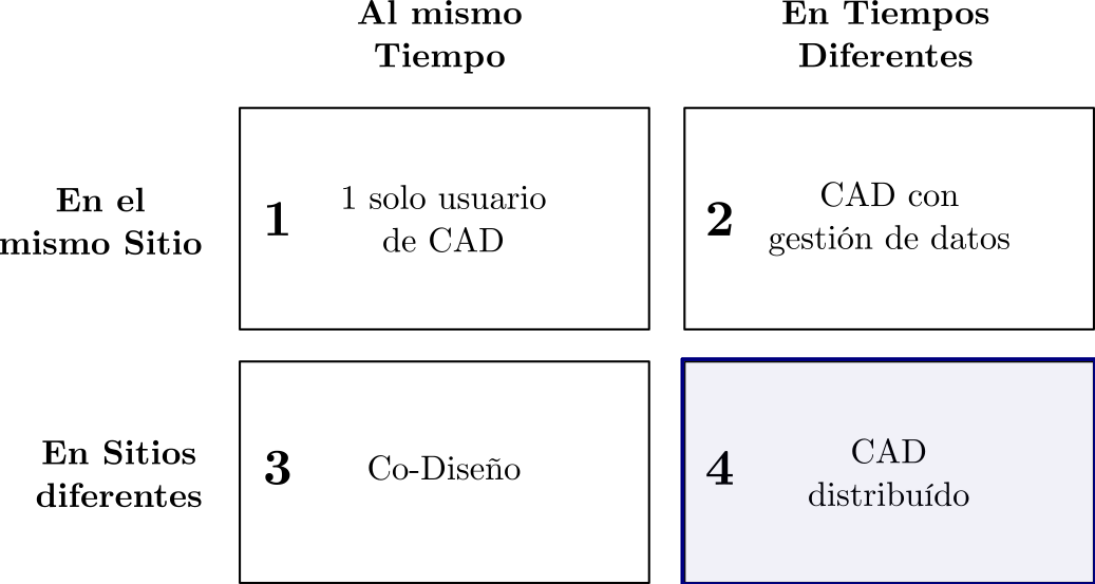
\includegraphics[width=10cm]{Img/CPD/cad-time.png}
\centering
\caption{\footnotesize{El uso del CAD en el espacio y tiempo}}
\label{fig:tablacad}
\end{figure}

El contenido compartido en los ambientes de \textbf{diseño colaborativo y distribuido} por lo general implica el uso de \textbf{modelos 3D} como medio de comunicación entre los participantes con el fin de visualizar ideas abstractas y se usan iterativamente durante todo el proceso de diseño \citep{Tek-JinNam2009}. Los participantes requieren diferentes vistas del diseño, pueden tener intereses diferentes respecto %desarrollo de 
a las soluciones y su representación asociada. De manera que, se necesitan múltiples niveles de abstracción en términos de soporte informático para gestionar la diversidad de conocimiento. %Además, para permitir la participación


\subsection{Soporte informático a la colaboración }
La colaboración se puede lograr mediante un \textbf{Espacio de Trabajo Compartido} en inglés \textit{\Gls{Shared Workspace}}  (ver figura \ref{fig:sistemashared}). 
Este proporciona una comunicación visual y funciona como un medio en el que un actor puede comprender el modelo/diseño de otro sin necesidad de tener el mismo vocabulario \citep{Maher2006}. 
Un espacio de trabajo compartido CAD se puede dividir en dos significados: El espacio de trabajo con el que los participantes humanos visualizan el diseño e interactúan y la representación compartida del problema de diseño que utiliza la propia computadora para la persistencia y la comunicación entre procesos. Por ende se consideran dos categorías de representaciones en el espacio de trabajo: \textbf{{Representación visual}} compartida y \textbf{Representación subyacente} compartida. Esto proviene de los requisitos de los sistemas multiusuario, en el que los usuarios puedan ver el trabajo de los demás. La parte visual es proporcionada por los modelos 3D y además con la posibilidad que el sistema mantenga una o más representaciones de la solución de diseño (versiones). Cualquier otro conocimiento de dominio relevante es proporcionado por el contenido subyacente, por ejemplo: referencias, documentación técnica, archivos extra para interactuar con otros sistemas, etc.

\begin{figure}[ht]
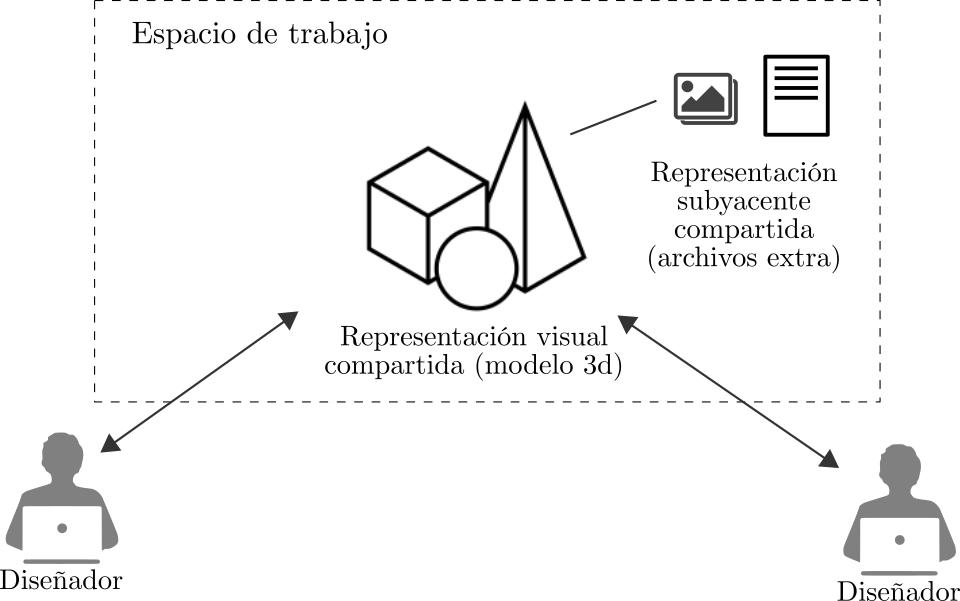
\includegraphics[width=10cm]{Img/CPD/cad-shared.png}
\centering
\caption{\footnotesize{Representaciones en un espacio de trabajo compartido.}}
\label{fig:sistemashared}
\end{figure}

Aparte de la implementación de un espacio compartido, resolver problemas como el modelado no es una tarea trivial para los sistemas y se necesita de una infraestructura y componentes con determinadas características. A continuación se explican los sistemas de modelado sólido.

\subsection{Sistemas de Modelado Sólido }

En la creación de un sistema de modelado de sólidos o ``modelador sólido'' se deben considerar las condiciones geométricas y topológicas explicadas en la sección \ref{ref:modelado-solido}. Mäntylä expone que la idea fundamental es separar el modelo geométrico de la aplicación y desarrollar técnicas de modelado que sean independientes de los objetos \citep{Mantyla:1988:ISM:60949}. Los pasos a dar se ilustran en la figura \ref{fig:sistema-solido} y pueden resumir de la siguiente manera:


\begin{itemize}
\item Inicialmente, 
los objetos son descritos por el usuario mediante un \textbf{lenguaje de descripción}, basados en los conceptos de modelado (poligonal, booleano, etc) aplicados al sistema. 
Se introducen utilizando \textit{scripting}, con lenguajes como OpenSCAD o \Gls{python}\footnote{\url{http://python.org}}, o bien mediante una \textbf{interfaz de usuario} para interactuar gráficamente. Un mismo sistema puede incluir varios lenguajes de descripción, atendiendo a diferentes usuarios y aplicaciones.

\item Una vez introducidos, los objetos son traducidos para crear la \textbf{representación interna} almacenada por el modelador. 
La relación entre el lenguaje de descripción y la representación interna no necesariamente debe de ser directa: las representaciones internas pueden emplear conceptos de modelado distintos a la descripción original. La transformación del lenguaje de descripción a la representación interna es necesaria para poder encontrar las respuestas a las preguntas geométricas. De hecho, para que un sistema de modelado sea eficiente, debe soportar múltiples representaciones internas de los objetos, por ejemplo con diferentes tecnologías para geometrías como \Gls{CGCAL}\footnote{\url{https://www.cgal.org/}} u \Gls{Open-Cascade}\footnote{\url{https://www.opencascade.com/content/latest-release}}. Por lo tanto, se deben incluir algoritmos de conversión que puedan modificar una representación en otra.

 \item Para comunicarse con otros sistemas de modelado  (importación/exportación) el modelador debe proveer interfaces de comunicación. 
 Estas interfaces son utilizadas para recibir o transmitir modelos hacia o desde otros sistemas de modelado. Necesariamente debe manejar información geométrica utilizando formatos existentes como por ejemplo \Gls{STEP} acrónimo de \textit{Standard for the Exchange of Product Data} \citep{Wilson1998} o \Gls{STL} acrónimo  de \textit{Stereolithography} \citep{grimm2004user}.

\item Finalmente, el modelador también debe incluir facilidades para almacenar las descripción de objetos y demás datos, en bases de datos permanentes. 
\end{itemize}

\begin{figure}[ht]
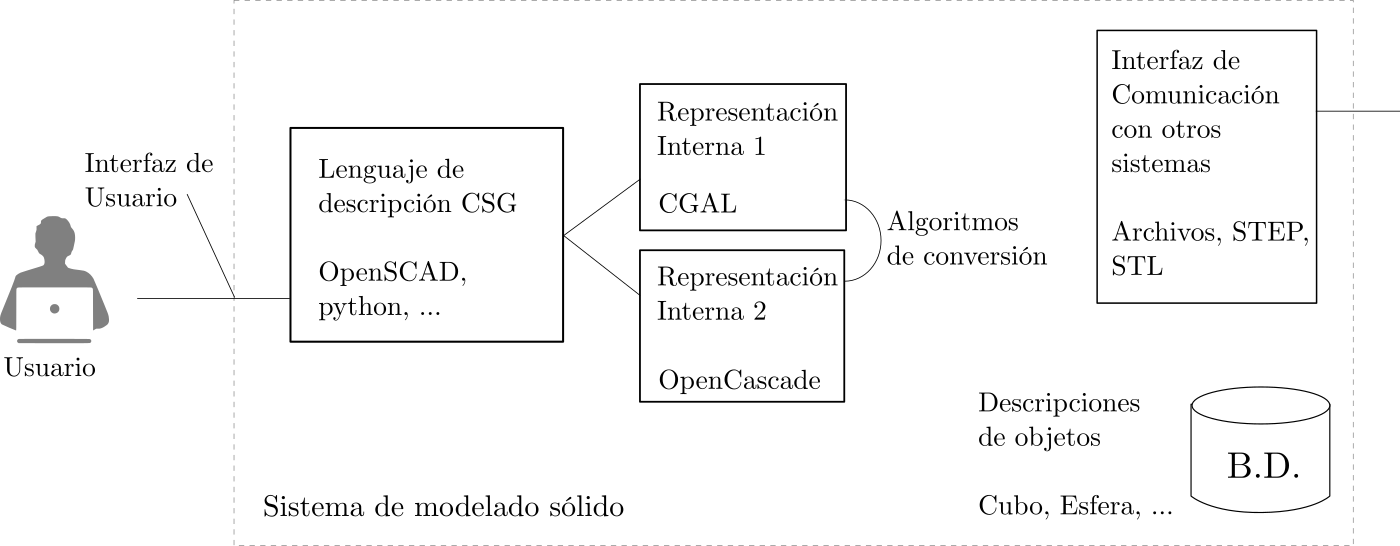
\includegraphics[width=14cm]{Img/GEO/sistema-solido.png}
\centering
\caption{ \footnotesize{Sistema de Modelado Sólido. 

%El usuario (izquierda) ingresa las descripciones de los objetos a través de la interfaz de usuario mediante un lenguaje de \textit{scripting} (OpenSCAD, python, etc). Luego, el lenguaje de descripción es traducido a la representación interna (GCAL, OpenCascade, etc) para encontrar las respuestas a las preguntas geométricas (centro). Si existen varias representaciones internas se utilizan los algoritmos de conversión. En la derecha se puede apreciar la Interfaz de Comunicación con otros sistemas y la Base de Datos permanente con las descripciones de los objetos (primitivas). \citep{Ramos2011}

}}
\label{fig:sistema-solido}
\end{figure}

En estos sistemas se pueden distinguir tres niveles de abstracción:

\begin{enumerate}
\item \textbf{Interfaz de usuario.} Mediante el lenguaje de descripción, el usuario utiliza las operaciones disponibles en cualquier aplicación CAD (crear, modificar, guardar, borrar y analizar diseños).
\item \textbf{Infraestructura matemática y algorítmica.}  Implementa las operaciones que proporciona el nivel anterior (por ejemplo, los algoritmos CSG para trabajar con objetos mediante operaciones booleanas).
\item \textbf{Primitivas.} A nivel de sistema, son operaciones aritméticas y lógicas que describen los objetos primitivos. Se encuentran disponibles de forma permanente en bases de datos para que puedan ser utilizadas por el nivel anterior.
\end{enumerate}

Dentro de la complejidad de un modelador es indispensable que los datos de los productos sean accesibles y carezcan de errores.
Para lograrlo se utilizan los sistemas de  \textbf{Gestión de Datos del Producto} en inglés \textit{Product Data Management} (\Gls{PDM}) \citep{Ruiz} los cuáles se explican a continuación.



\subsection{Gestión de Datos del Producto (PDM)}
\label{sec:pdm}
Max Ungerer define que \textquote{\textit{un sistema PDM es ``algo'' que maneja datos sobre productos}}. En el núcleo central de la información está la identificación del producto y se representa conceptualmente como un elemento o ítem dentro del sistema \citep{Ungerer2002}. \vskip


Para garantizar la colaboración distribuida, los PDM tradicionales tienen los mismos problemas que las aplicaciones de escritorio:

\begin{enumerate}
    \item {Es difícil proporcionar acceso a los usuarios desde diferentes ubicaciones}, especialmente aquellos que se encuentran en diferentes redes. En cada implementación del PDM, las configuraciones de red deben ser homogéneas. 
    \item {Las aplicaciones cliente\footnote{El cliente es una aplicación informática  que consume un servicio remoto} son dependientes de la plataforma}, todos los usuarios deben usar la misma plataforma informática o bien se debe proporcionar una aplicación específica para cada plataforma de usuario. Actualmente, es casi imposible este mandato por la diversidad de sistemas y dispositivos. 
    \item {Las tareas de ampliación y actualización no son sencillas}, cuando se requieren nuevas funciones, los usuarios deben volver a instalar o actualizar la aplicación completamente. 
\end{enumerate}

En consecuencia, es lógico utilizar un \textbf{PDM basado en la web} en inglés \textit{Web based Product Data Management} (\Gls{WPDM}) \citep{Huang2004} porque pueden ofrecer soluciones centradas en la lógica de negocio de las empresas y proporcionar una comunicación global sin mucho esfuerzo, brindando funciones independientes de las redes y la plataforma. Esto se traduce en una reducción del costo general para la implementación. Un WPDM eficiente requiere:
\begin{itemize}
    \item Ser totalmente escalable para proporcionar flexibilidad, porque cada organización tiene diferentes prioridades y diferentes flujos de trabajo.
   \item Ser sencillo de usar por todos los participantes.
    \item Tener una arquitectura abierta para que se permite añadir, modernizar y cambiar sus componentes sin depender de un proveedor.
    \item Estar disponible en una amplia variedad de plataformas y proveer funciones en redes heterogéneas.
\end{itemize}

La mayoría de los sistemas WPDM que se han implementado con éxito hacen uso de \textbf{Servicios Web} en inglés  \textit{\Gls{Web Services}} \citep{richardson2008restful}.


\subsection{Intercambio de datos CAD}
En el pasado, el proceso de intercambio de datos estaba relacionado con los planos y los documentos técnicos, actualmente se requieren archivos digitales  compartidos entre múltiples aplicaciones.
Los esfuerzos hacia la integración del CAD generaron 
el desarrollo de varios formatos estándares para el \textbf{Intercambio de Datos de CAD} en inglés \textit{CAD Data Exchange} \citep{Randjelovic2007}, así como muchos ``no estándares". Los formatos han variado desde archivos para datos de dibujo técnico como DXF\footnote{\url{https://es.wikipedia.org/wiki/DXF}} hasta representaciones de modelos 3D como STEP \citep{Wilson1998}. 

En lo ámbitos de fabricación digital el \textit{CAD Data Exchange} es la norma, a pesar de que cada sistema tiene su propio formatos de datos. Así, la misma  información puede ser ingresada varias veces en diferente sistemas, provocando redundancia.   
Además, el uso de modelos 3D de geometría compleja puede provocar errores en los datos de diseño, con  representaciones incorrectas y falta de entendimiento entre los actores. Respecto a esta problemática, desde el año 1999 el Instituto Nacional de Estándares de EE.UU.  (NIST)\footnote{\url{https://www.nist.gov/}} estima que la incompatibilidad de datos se traduce en costos que alcanzan los 90 millones de dólares por año  \citep{Tassey1999}. \vskip

En conclusión, el \textit{CAD Data Exchange} es fundamental en el contexto actual del modelado geométrico, ya que es el mecanismo principal para lograr interoperabilidad la entre las diferentes plataformas.

\subsubsection{Data Exchange Geométrico}


El enfoque establecido para el intercambio de datos se denomina \textbf{Data Exchange de la geometría} o \textbf{\Gls{DE} geométrico} \citep{Spitz:2004:IFG:1217875.1217904}, en este la representación del objeto se transfiere de un sistema origen a un sistema de destino. En las aplicaciones comerciales se implementan a través de los \textbf{formatos neutrales} que pueden ser generados y leídos en la mayoría de los sistema CAD. Algunos ejemplos de ellos son STEP y STL, acrónimo  de \textit{STereoLithography} \citep{grimm2004user}. 
\vskip
STEP interpreta un producto como uno o varios documentos. Utiliza \textbf{grupos de conceptos} para organizar los elementos de manera lógica y así generar una estructura clara y comprensible para todas las plataformas. Su estructura depende de la dirección que tome el sistema PDM, sus protocolos de aplicación y su alcance. \vskip 

Por su parte, los archivos STL describen la geometría de un objeto 3D mediante triángulos, sin considerar la representación de color, textura u otros atributos. Se pueden especificar tanto en \Gls{ASCII} como en binario y se caracterizan por ser ampliamente utilizados para fabricación digital. 
\vskip 


El uso del DE geométrico con formatos neutrales o nativos es bastante confiable, aunque muchas veces es posible obtener resultados de modelos no sólidos debido a la perdida de información de sus estructuras.
No obstante, su principal inconveniente no es la inconsistencia geométrica, sino el hecho de que no es compatible con el paradigma de diseño más común de la actualidad: el diseño \textbf{basado en características} en inglés \textit{Feature Based} (\Gls{FB}), también llamado \textbf{diseño paramétrico} o \textbf{diseño basado en la historia} como se explica en la sección \ref{cadparam}.
Por esa razón es imposible realizar modificaciones de los modelos en el lado del sistema destino. Esta situación se puede ver ilustrada en el ejemplo de la figura \ref{fig:de0}. El usuario en el sistema origen (izquierda) puede visualizar y modificar el modelo para compartir con el sistema destino mediante un archivo en formato STEP que incluye los datos geométricos. Por otra parte el usuario en el sistema destino (derecha) puede visualizar el modelo pero no modificarlo, puesto que solamente tiene acceso a los datos geométricos, pero no a los parámetros necesarios para alterar la representación. 

\begin{figure}[ht]
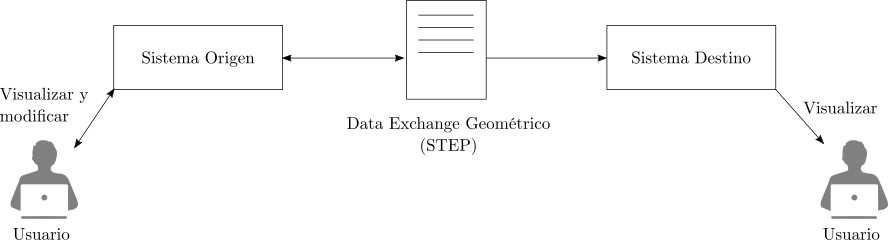
\includegraphics[width=14cm]{Img/WEB/de0.png}
\centering
\caption{\footnotesize{Esquema de Data Exchange Geométrico. 
}}
\label{fig:de0}
\end{figure}

De esta limitación surge el  \textbf{Intercambio de Datos Basado en Características} en inglés \textit{Feature Based Data Exchange} (\Gls{FBDE}) \citep{Spitz:2004:IFG:1217875.1217904}.

\subsubsection{Data Exchange basado en características (FBDE)}
\label{FBDE}

En el FBDE, dado un grafo o estructura  basada en el historial paramétrico de un modelo (características) en un sistema origen, el objetivo es construir un grafo en un sistema destino con una geometría similar, conservando al mismo tiempo la mayor información paramétrica posible. En muchos casos, la geometría puede no ser idéntica debido a diferentes políticas de tolerancia entre los sistemas CAD. Siempre que la aproximación esté controlada es totalmente aceptable en la práctica. \vskip
El FBDE conserva la inteligencia del diseño, permitiendo que se realicen modificaciones en el lado del sistema destino (ver figura  \ref{fig:de1}). El usuario en el sistema origen (izquierda) puede visualizar y modificar el modelo. La compartición del modelo se realiza mediante un formato o tipo de fichero que contiene los datos geométricos y también expone las características del modelo mediante los parámetros. En el sistema destino (derecha) se puede visualizar y manipular el modelo debido a que posee los datos geométricos y paramétricos para modificar la representación. 

\begin{figure}[ht]
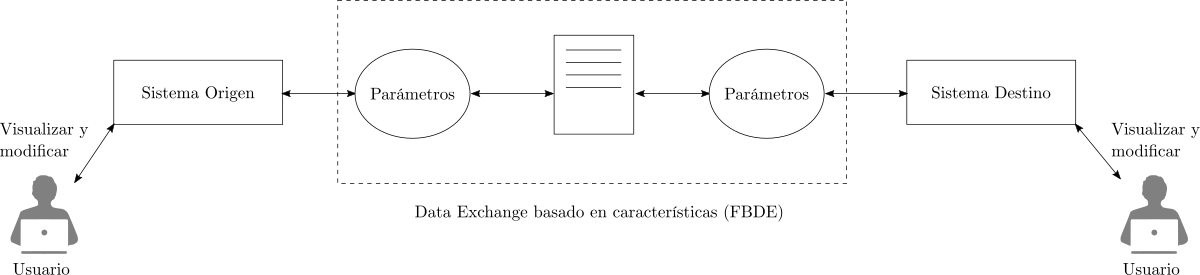
\includegraphics[width=16cm]{Img/WEB/de1.png}
\centering
\caption{\footnotesize{Esquema de Data Exchange basado en características (FBDE). }}
\label{fig:de1}
\end{figure}

Adicionalmente, el sistema debe contar con mecanismos para evitar o reparar problemas de inconsistencias geométricas en los archivos de intercambio.\vskip
El modelo se suele representar como un árbol o lista de operaciones, comúnmente llamado \textbf{árbol de historia}. Las operaciones crean una nueva geometría o modifican una existente. Esta estructura se puede considerar una extensión de la geometría constructiva de sólidos (CSG) explicada en la sección \ref{mod:booleano}. El punto principal de este paradigma es que las operaciones son siempre de naturaleza paramétrica. 

En la figura \ref{fig:de2} se ilustra un ejemplo con las diferentes versiones de un modelo mecánico (derecha) y su representación como árbol de historia (FBDE) (izquierda). Las versiones se producen a partir de las operaciones o modificaciones de los parámetros, desde un \textbf{modelo original} hasta un \textbf{modelo objetivo}. En cada nivel del árbol se pueden ver las operaciones realizadas.  Partiendo del modelo original, para obtener la \textit{Versión \#1} se modifica el parámetro \textit{cilindros\_B = 0} a \textit{cilindros\_B = 8} de manera que se agregan 8 cilindros. Esta operación genera una separación entre la pieza y los cilindros, produciendo un objeto ``no sólido''. La \textit{Versión \#2} soluciona este problema, convirtiendo al objeto nuevamente en sólido con la modificación de la variable \textit{cilindros\_A = 8} y su correspondiente incorporación de 8 cilindros de base. Finalmente a la \textit{Versión \#2} se aplica un operador booleano de  intersección entre el modelo y un cilindro, generando un orificio en el modelo objetivo 
\citep{Kwon2015}.

\begin{figure}[ht]
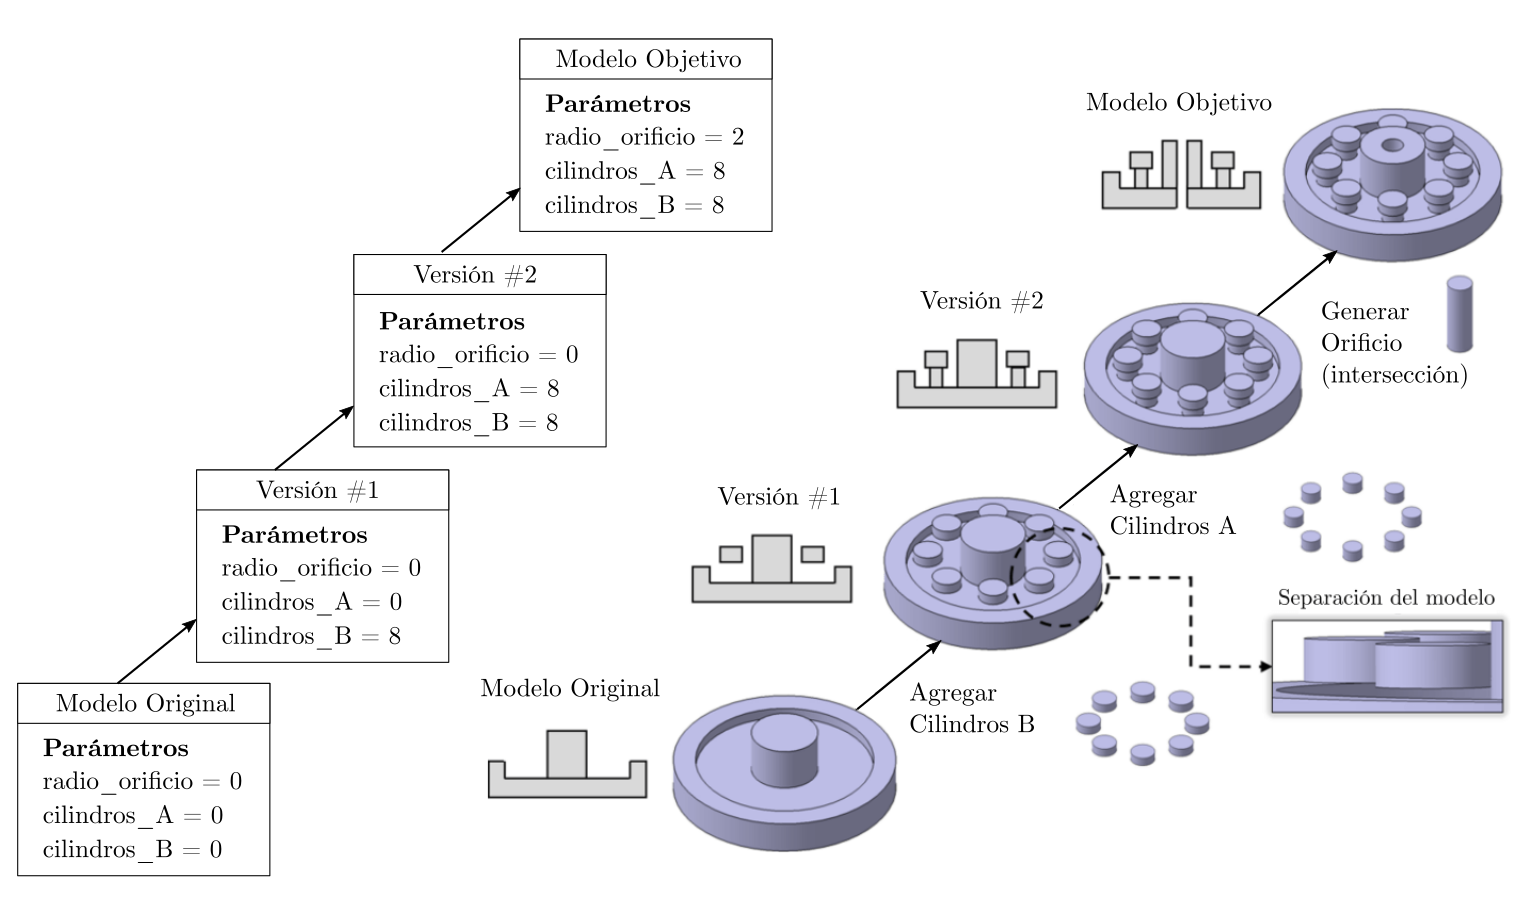
\includegraphics[width=16cm]{Img/WEB/de-fin.png}
\centering
\caption{\footnotesize{ Modelo mecánico y su representación como árbol de historia (FBDE). }}
\label{fig:de2}
\end{figure}



Por lo anteriormente expuesto, es deseable un sistema de \textbf{CAD distribuido} que permita el \textbf{co-diseño} de productos orientados a la \textbf{fabricación digital}, este debe tener capacidades para la  gestión de datos de productos basados en la web \textbf{(WPDM)} y soporte al intercambio de datos basados en características \textbf{(FBDE)}.

Para que el desarrollo del sistema esté en sintonía con los principios colaborativos planteados, se pueden utilizar metodologías o enfoques orientados a la experiencia de usuario (UX) como \textit{Lean UX}.  

%\clearpage
\section{Lean UX}
\label{section:pmv}
Los equipos de desarrollo de software son un ejemplo de eficiencia en la colaboración, utilizan técnicas de desarrollo ágil \citep{cockburn2002agile}, reduciendo drásticamente el tiempo que requiere modificar una aplicación, realizan cambios en el código y 
lo llevan a producción\footnote{Producción es la instancia del software cuando se encuentra a disposición de los usuarios finales.} a una velocidad similar a la de guardar un archivo en un ordenador. Además,  utilizan mecanismos para iterar incorporando lo que han aprendido y tal vez, sin advertirlo, aumentan las expectativas de los usuarios.  \Gls{GitHub}\footnote{\url{https://github.com/}} es un caso de éxito como plataforma de trabajo colaborativo, convirtiéndose en la herramienta de gestión de código más utilizada en la actualidad \citep{GitHub2018}.
En este nuevo contexto, las prácticas de analizar todo el proyecto al inicio quedaron obsoletas. \vskip
\textit{Lean User Experience} (Lean UX) \citep{Gothelf2013} 
es una metodología que utiliza las herramientas disponibles y las combina de forma diferente para adecuarlas a esta nueva realidad. Jeff Gothelf y Josh Seiden la describen como \textquote{\textit{una nueva etapa evolutiva en el diseño de productos}}. 
Se considera profundamente colaborativa y multidisciplinaria, en gran medida porque permite implementar técnicas para construir una comprensión compartida del proyecto, logra un ambiente propicio para el \textit{\gls{feedback}} con los usuarios finales, replantea las conversaciones de diseño en términos objetivos y cambia la forma en que se comunica el diseño del producto: en lugar de hablar de funciones y documentos, se habla de lo que efectivamente funciona y de lo que no.


\vspace{5mm}

Los \textbf{3 pilares principales de Lean UX} son:
\begin{enumerate}
    \item \textbf{Design Thinking o Pensamiento de Diseño} \vskip
    
    El \textit{Design Thinking} \citep{Brown2009} logra obtener soluciones involucrando a los usuarios para convertirlos en actores activos en todo el proceso de la construcción del producto. 
    Es una manera de trabajar que alienta la colaboración del  equipo, independientemente del rol que cada actor desempeñe. Centra su eficacia en entender y dar solución a las necesidades reales de los usuarios.

    \item \textbf{Metodologías de desarrollo ágil de software}.\vskip
    Los desarrolladores de software las han usado durante mucho tiempo.
    No obstante, estas  constituyen un reto para los diseñadores. \textit{Lean UX} aplica los 4 principios básicos del desarrollo ágil al diseño de productos \citep{Gothelf2013} :
        
        \begin{enumerate}
        \item
        \textbf{Los individuos y las interacciones son más importantes que los procesos y las herramientas}: 
        Para generar rápido las mejores soluciones, se debe implicar a todo el equipo. 
        La comunicación fluida  debe primar por encima de las restricciones propias de las herramientas.
        \item
        \textbf{El software funcional es más importante que la documentación exhaustiva}: 
        Un software que funcione es más importante que preocuparse por una documentación exhaustiva. De esta manera, se puede encontrar de antemano la solución que mejor se adapte a las necesidades.
        \item
        \textbf{La colaboración con los clientes es más importante que la negociación de contratos con ellos}: 
        Si el equipo colabora con los usuarios/clientes, hay un entendimiento común sobre los problemas y las posibles soluciones. Cualquier decisión se debe tomar por consenso, esto se traduce en iteraciones más rápidas y una verdadera implicación de todos los actores con la ventaja de trabajar siempre con soluciones validadas. 
        \item
        \textbf{La respuesta a los cambios es más importante que la planificación}: 
        Se asume que el equipo no encontrará la solución la primera vez, por lo que el objetivo consiste en averiguar en que se ha fallado. Luego se pueden ajustar las propuestas y volver a probarlas iterativamente. 
        \end{enumerate}

\item \textbf{Método Lean Startup}\vskip 

Los proyectos han estado enmarcados, tradicionalmente, por los requerimientos y las entregas. A los equipos se les suministraban requerimientos para que produjeran entregas.
No se inicia a partir de requerimientos, sino de  suposiciones. A partir de ellas, se crean y prueban \textbf{hipótesis} o \textquote{una manera de expresar las suposiciones que se tienen del proyecto de una forma comprobable} \citep{Gothelf2013}. 

\textit{Lean Startup} \citep{ries2012metodo} utiliza un ciclo de \textit{feedback} denominado \textbf{``construir-medir-aprender''} que minimiza el riesgo de los proyectos y  consigue que el equipo pueda desarrollar software y aprenda de él en muy poco tiempo (ver figura \ref{fig:ciclolean}). Consiste en poner en marcha (construir) las ideas que se suponen van a tener éxito, medir y recabar los datos para confirmar o desmentir las hipótesis que se plantearon al principio y aprender del fracaso o el éxito resultante. En el centro de la figura se aprecia la interacción entre las ideas, el producto construido (\Gls{PMV}) y los datos recabados \citep{Borodin2018}.

\begin{figure}[h]
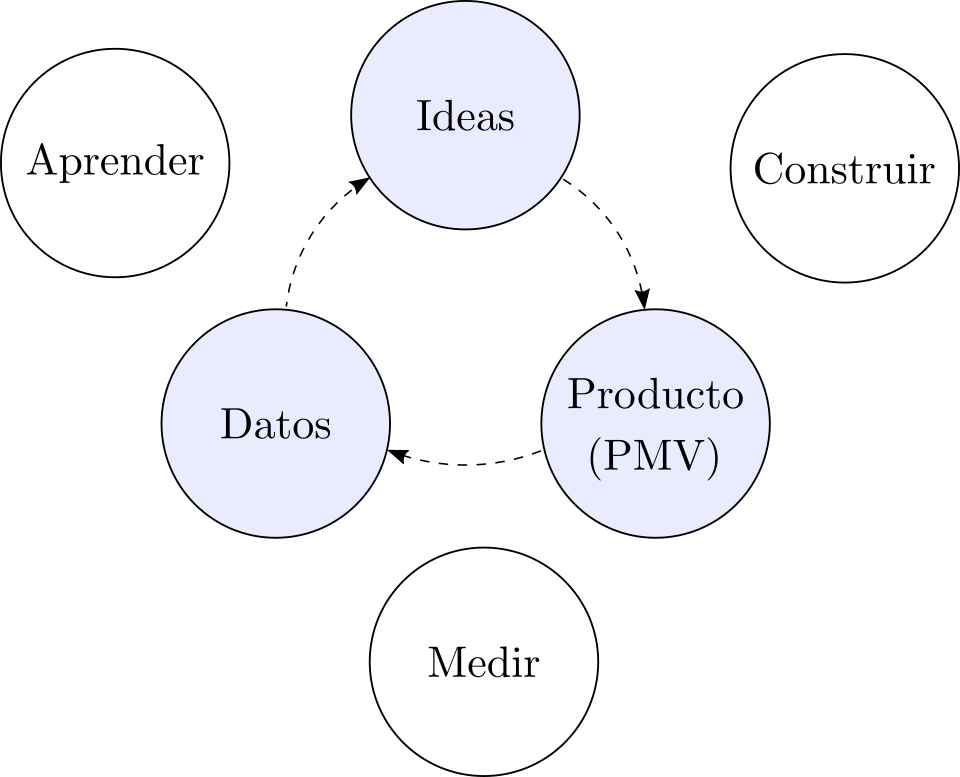
\includegraphics[width=7cm]{Img/Desarrollo/lean1.png}
\centering
\caption{\footnotesize{Ciclo Construir-Medir-Aprender.}}
\label{fig:ciclolean}
\end{figure}


De esta manera, los equipos pueden desarrollar de inmediato los denominados \textbf{Productos Mínimos Viables} (PMV) en inglés \textit{Minimum Viable Products} (MVP) \citep{olsen2015lean}. El ciclo se desarrolla de la siguiente manera:


    \begin{itemize}
    \item En primer lugar, se construye un PMV, es decir, \textbf{el desarrollo más pequeño que pueda construirse para probar cada hipótesis}. Se debe tener en cuenta que tanto el PMV inicial como las siguientes iteraciones deben tener valor por sí mismas. Es decir, se debe obtener un \textit{feedback} del usuario final. Para esto, el producto debe tener el mismo tratamiento utilizado en el diseño iterativo. Para un mejor entendimiento de este punto, se puede analizar la figura \ref{fig: incremental} explicada en la sección \ref{iterativo}.
    

    \item El siguiente paso es entregar el PMV a los usuarios y realizar experimentos que puedan ser medidos para obtener datos.
    \item Después, se utiliza lo aprendido con ellos para evaluar las hipótesis y hacer las modificaciones pertinentes.
    \item Y finalmente se itera, se comienza todo el proceso nuevamente. 
    \end{itemize} 


\end{enumerate}

%\clearpage
\subsubsection{Proceso Lean UX}
El objetivo final es trasladar todos los valores heredados de los 3 pilares al trabajo de experiencia de usuario mediante un conjunto de pasos definidos, métodos y herramientas que se analizan a continuación.

\begin{figure}[h]
    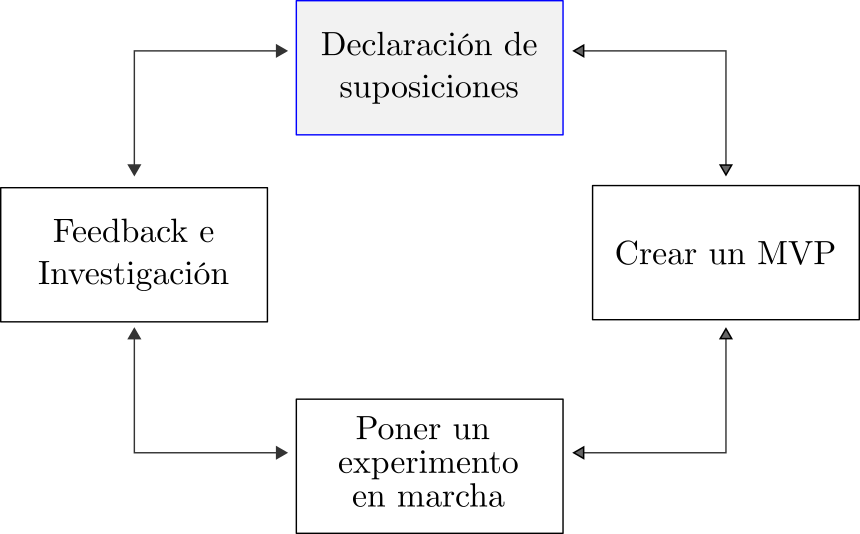
\includegraphics[width=9cm]{Img/Desarrollo/desarrollo1.png}
    \centering
    \caption{\footnotesize{Proceso Lean UX. }}
    \label{fig:leanux1}
\end{figure}
    
\subsubsection{Declaración de suposiciones}
Antes de cualquier declaración, se realiza una exploración  recurriendo a técnicas de investigación en inglés \textit{\gls{research}} \citep{sharon2016validating} sobre los usuarios y sus necesidades. Estas declaraciones se componen de los siguientes elementos:


\begin{itemize}
    \item \textbf{Suposiciones}: una declaración de alto nivel que se considera cierta. 
    El primer paso en \textit{Lean UX} es declarar las suposiciones (ver figura \ref{fig:leanux1}), este ejercicio se realiza en equipo,  asegurándose de que todas las disciplinas estén representadas. Con toda la información recolectada se continúa con la declaración del problema.
    
    \textbf{Método: Declaración de problema}\vskip
    \label{sec:dec-problema}
    Permite centrar correctamente el trabajo de todo el equipo y  define las restricciones y límites necesarios para que no se pierda  de vista el objetivo. Se puede utilizar la siguiente plantilla:
    \textquote{[El servicio/producto] debe cumplir con [estos objetivos]. Sin embargo, se ha observado que no se están alcanzando [estos objetivos], lo que está causando [este efecto adverso] para los usuarios. ¿Cómo se podría mejorar el  [servicio/producto] de modo que los usuarios consigan mejorar sus resultado según [estos criterios cuantificables o cualificables]?}\vskip
    
    Generalmente las declaraciones está repletas de suposiciones, para extraerlas se utiliza una lista u \textbf{hoja de suposiciones}.

En base a las siguientes preguntas, se recopilan las declaraciones que reflejen lo que el equipo de desarrollo considere cierto respecto a la solución o producto. 
\textbf{¿Quiénes son los usuarios del producto?  
¿Cómo encaja en su trabajo? 
¿Qué problemas soluciona? 
¿Cuáles son sus funciones más importantes? ¿Qué aspecto debe tener y cómo debe comportarse?}

Si existen diferencias en un punto, lo mejor es reflejar esto de inmediato para facilitar la discusión entre los miembros del equipo de desarrollo. Una vez obtenida la lista de suposiciones priorizada, es necesario probarlas. 
    
    \item \textbf{Hipótesis}: descripciones más detalladas de las suposiciones, dirigidas a áreas específicas del producto o flujos de trabajo 
    con las que se puede experimentar.
Es decir, se transforman las suposiciones
a un formato más sencillo de probar.
Sin embargo, las hipótesis suelen ser demasiado extensas para que, con una única prueba, se pueda determinarse su validez. Contiene demasiadas partes, es decir, demasiadas ``sub-hipótesis''. Para 
registrar estas partes más pequeñas y específicas se utiliza la siguiente plantilla: \vskip

\textquote{Se considera que [haciendo esto, desarrollando esta función, creando esta experiencia de usuario] para [estas  personas] se conseguirá [este resultado]. 
Se sabrá si esto es correcto cuando se obtenga [esta medida cuantitativa, o este conocimiento cualitativo]}.\vskip 

El primer campo se completa con la función o mejora para el producto. El segundo describe exactamente qué usuarios objetivo se beneficiarán de la función. El último, especifica los beneficios que esos usuarios obtendrán de ella. La frase final lo une todo. Esta frase determina si la hipótesis es cierta o no.

    \item \textbf{Resultados}: los datos de entrada, proveniente de la experiencia de los usuarios, que ayudan a validar o invalidar las hipótesis. Pueden ser cuantitativos o  cualitativos.
    En principio se encuentran con resultados de alto nivel o generales. Se debe considerar cómo dividir esos resultados en componentes más pequeños, 
    específicos y cercanos a la realidad del proyecto.
    ¿Qué funciones en la UI podrían generar un mayor uso? ¿Un visor 3D totalmente funcional o simplemente compartiendo imágenes? Mediante estas preguntas, se enuncian resultados que se acercan a las necesidades reales del proyecto. Ejemplo: \textbf{Dar soporte a la visualización de modelos 3D en la web}.
    
    \item \textbf{Personas}: son modelos o arquetipos \citep{Gothelf2013} de los potenciales usuarios  para las que se considera estar resolviendo el problema.
    Detallan quién utilizará el producto y por qué lo hará. Se inicia con esquema muy sencillo, en cuya creación participa todo el equipo. A medida que se avanza en la investigación se pueden realizar ajustes.\vskip
    
    \item \textbf{Funciones o funcionalidades}: son las técnicas, las funciones, los productos y los servicios a desarrollar para conseguir los resultados. Normalmente, en este punto todos los miembros del equipo tienen su propia opinión, ya que, después de todo, las funciones son lo más concreto con lo que trabajan y les resulta más sencillo expresar sus ideas en términos de funciones. Sin embargo, un error común es hacer que el proceso de diseño parta de las funciones.
    
    

    Con todo el material obtenido se organizan las sub-hipótesis que deben probarse en una \textbf{tabla de sub-hipótesis}. La tabla se organiza con el siguiente formato: Función / Persona / Resultado.

\end{itemize}

\subsubsection{Diseño Colaborativo}

\label{dis-colabo}
 Con la \textbf{tabla de sub-hipótesis} como guía se reúne a diseñadores y no diseñadores (programadores, administradores de proyectos) 
 para crear los conceptos del producto 
 , y un entendimiento común sobre el problema y las soluciones de diseño. 
 Asimismo, permite decidir qué  elementos de la interfaz gráfica implementan mejor las funciones recogidas en las hipótesis.
 A continuación se describen dos herramientas utilizadas para el diseño de interfaces.
 
 \begin{itemize}
     \item \textbf{Estudio de diseño}: 
    \textquote{\textit{Un equipo interdisciplinario se reúne en una sesión de trabajo o \textbf{Estudio de Diseño} (a veces también llamado Charrette de diseño)}}\citep{Gothelf2013}. Permite explorar y analizar qué elementos de la interfaz gráfica pueden implementar mejor las funciones recogidas en las hipótesis.
    La documentación de salida de las sesiones constan normalmente de \textbf{esquemas de baja fidelidad} en inglés \textit{\gls{Sketch}} (ver figura \ref{salida}). Es esencial que la documentación no sea muy elaborada para que el trabajo continúe siendo maleable. De esta manera, el equipo puede cambiar de dirección con facilidad si las pruebas demuestran que el enfoque adoptado no es el correcto.
    \item \textbf{Guía de estilo}: 
    \label{style}
    En base a la documentación resultante del estudio de diseño se desarrolla la \textbf{guía de estilo}, una biblioteca de patrones aceptada por todo el equipo, para codificar los elementos gráficos e interactivos de la interfaz de usuario. También sirve para recopilar los componentes web en inglés \textit{\Gls{Web Components}}\footnote{\url{https://www.webcomponents.org/introduction}} del producto, todo lo que forme parte de la experiencia de usuario (UX) aparece en la guía de estilo. No solo se define el aspecto y el comportamiento, sino que también se proporciona la codificación de los componentes y las hojas de estilo en inglés \textit{Cascading Style Sheet} (\gls{CSS})\footnote{\url{https://www.w3.org/Style/CSS/}}. De esta manera, al modificar la guía de estilo también se modifica el producto. 
    
    \end{itemize}
 

\subsubsection{PMV y experimentos}

\label{pmv-cocada}
Con la lista de sub-hipótesis  se crean los PMV, explicado en la sección \ref{section:pmv}. Se utilizan para hacer experimentos y determinar qué ideas sobre el producto son válidas y cuáles deben descartarse.
Una de las maneras más efectivas de crear los PMV es mediante un prototipo de la experiencia. \textquote{\textit{Un prototipo es una aproximación de la experiencia de usuario que permite simular cómo será el uso de un producto o servicio}} \citep{Gothelf2013}. Es recomendable probar el PMV en primera instancia con todo el equipo de desarrollo, y luego con otras personas. Cuánto más se exponga a las miradas ajenas, más conocimiento se tendrá para validarlo. El siguiente paso es la experimentación de los usuarios finales. La idea es dejar que lo utilicen libremente, 
así se puede obtener todo el \textit{feedback}
posible sobre la experiencia.\vskip

\subsubsection{Feedback}
Hasta ahora, todo el trabajo está basado en las suposiciones; a partir de este punto se comienza con el proceso de validación. 
Un error común es realizar este proceso pocas veces, normalmente al principio del proyecto o al final.
La investigación es continua, lo que significa que se realizan en cada \textit{sprint} o iteración del producto.



Como consecuencia de usar este enfoque se obtiene: un equipo que trabaja de forma colaborativa, iterativamente, reduciendo al mínimo los documentos entregables, enfocándose en el software funcional y en el \textit{feedback} con el usuario final.


\section{Antecedentes}
\subsubsection{Speckle}
\Gls{Speckle} \citep{TheBartlett2015} comenzó como una investigación de diseño colaborativo para arquitectura en \textit{The Bartlett School of Architecture} (UCL)\footnote{\url{https://www.ucl.ac.uk/bartlett/architecture/}}.
El proyecto permite que los usuarios puedan compartir diseños paramétricos en la web. En la figura \ref{fig:spekle} se puede ver un modelo paramétrico en la plataforma web Speckle, a la izquierda se pueden apreciar los parámetros del modelo \citep{Dimitrie2017}. \\
El proyecto consta de:
\begin{itemize}
    \item Un plugin denominado \textit{Speckle Streams}\footnote{\url{https://www.food4rhino.com/app/speckle-streams}}  para el ecosistema del software  Rhino\footnote{\url{https://www.rhino3d.com/}}, este permite establecer los parámetros de los modelos y exportarlos a archivos en un formato específico.
    \item Una plataforma web que permite subir los archivos generados por el plugin para visualizar modelos 3D paramétricos, generar versiones modificadas, registrar un historial de los cambios y colaborar con otros usuarios.
\end{itemize}

\begin{figure}[h]
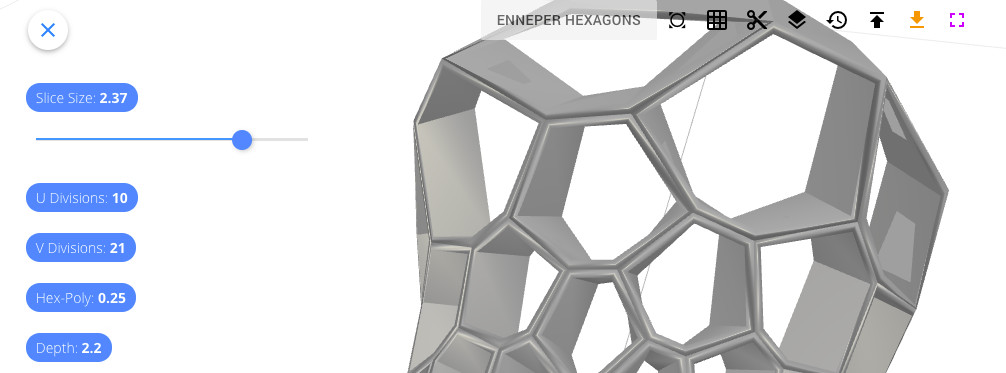
\includegraphics[width=14cm]{Img/Desarrollo/speckle.jpg}
\centering
\caption{\footnotesize{Interfaz web de Speckle.}}
\label{fig:spekle}
\end{figure}

Lo destacado de esta plataforma es la manera intuitiva de visualizar y modificar los modelos mediante su interfaz con componentes visuales como campos de texto, deslizadores, etc. \textbf{Speckle.Works}\footnote{\url{https://github.com/speckleworks}} es el repositorio FLOSS del proyecto que permite contribuciones de la comunidad. Actualmente se desarrollan diversas herramientas para la integración con otros softwares como Blender. 


\subsubsection{Modelo.io}
 Es una plataforma web creada por Qi Su y Tian Deng  \citep{Modelo.io2018} orientada a profesionales que utilizan Rhino y SketchUp\footnote{\url{https://www.sketchup.com/es}}. La característica de esta herramienta es que permite una colaboración efectiva entre los miembros de un equipo para perfeccionar los diseños y presentarlos de forma interactiva.

Los usuarios pueden explorar los modelos 3D, realizar comentarios, capturas de pantalla, anotaciones sobre los modelos, almacenar archivos extras asociados a los proyectos y otras características avanzadas como crear presentaciones 3D interactivas para los clientes. 
Se utiliza principalmente en   proyectos de arquitectura y diseño de interiores (ver figura \ref{fig:modelo.io}). En la interfaz web de \Gls{Modelo.io}, a la derecha se puede apreciar la interacción entre los usuarios \citep{Anthony2016} en un proyecto de arquitectura.

\begin{figure}[h]
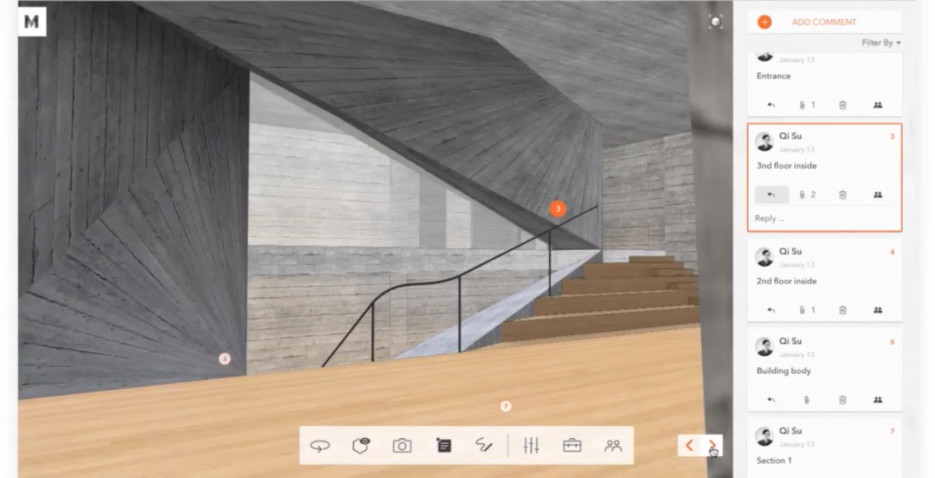
\includegraphics[width=14cm]{Img/Desarrollo/modeloio.jpg}
\centering
\caption{\footnotesize{Interfaz web de Modelo.io.}}
\label{fig:modelo.io}
\end{figure}




%\subsubsection{Problemas encontrados}
%En este trabajo se han presentado herramientas que soportan características relacionadas con el modelado especificado en algoritmos y la colaboración mediante modelos 3D. Los entornos analizados que permiten el modelado en la web son: OpenJSCAD y OnShape. Por otro lado, los entornos colaborativos son OnShape, Spekle.works y Modelo.io.
%En cierta medida, OnShape es la herramienta que cumple con los requisitos deseables para un sistema CAD distribuido vistos en la sección \ref{section:colabo}, sin embargo, presenta el problema de no ser intuitiva para aquellos usuarios que no cuentan con conocimientos en diseño mecánico avanzado o ingeniería como se puede apreciar en sus características principales\footnote{\url{https://www.onshape.com/}}. Dado que uno de los objetivos de este trabajo es lograr la colaboración entre personas con diferentes competencias, se debe abordar la solución teniendo presente este problema.